%\documentclass[handout]{beamer} % use this to disable \pause commands
\documentclass{beamer}
%
% Choose how your presentation looks.
%
% For more themes, color themes and font themes, see:
% http://deic.uab.es/~iblanes/beamer_gallery/index_by_theme.html
%
\mode<presentation>
{
  \usetheme{default}      % or try Darmstadt, Madrid, Warsaw, ...
  \usecolortheme{default} % or try albatross, beaver, crane, ...
  \usefonttheme{default}  % or try serif, structurebold, ...
  \setbeamertemplate{navigation symbols}{}
  \setbeamertemplate{caption}[numbered]
  \setbeamertemplate{footline}{% 
    \hfill% 
    \usebeamercolor[fg]{page number in head/foot}% 
    \usebeamerfont{page number in head/foot}% 
    \insertframenumber%
    %\,/\,\inserttotalframenumber
    \kern1em\vskip2pt% 
  }
} 

\usepackage[english]{babel}
\usepackage[utf8x]{inputenc}
\usepackage{pdfcomment}
\usepackage{fancyvrb}
\usepackage{tabularx}

\newcommand{\pdfnote}[1]{\marginnote{\pdfcomment[icon=note]{#1}}}

\newcommand\mydots{\hbox to 1em{.\hss.\hss.}}

\title[Your Short Title]{Concurrent Programming with\\Actors and Microservices}
\author{Maximilian Irro}
\date{Seminar für DiplomandInnen\\5.11.2018}

\begin{document}

\begin{frame}
  \titlepage
\end{frame}

% Uncomment these lines for an automatically generated outline.
%\begin{frame}{Outline}
%  \tableofcontents
%\end{frame}


\section{Concurrency}

% TODO hier sollte vielleicht noch ein anderer Slide vorher stehen

% ###################################################################

\begin{frame}{Forms of Concurrent Execution}

\begin{itemize}
  \pause
  \item \textbf{Pseudo-Simultaneous}: in alternation on a single CPU
  \pause
  \item \textbf{Parallel}: truely simultaneous on several CPU cores
  \pause
  \item \textbf{Distributed}: several host machines
\end{itemize}

\end{frame}

% ###################################################################

\begin{frame}{Foundational Issues of Concurrent Programming}

\begin{itemize}
  \pause
  \item \textbf{Expression of concurrent execution}: threads, futures, coroutines, etc.
  \pause
  \item \textbf{Communication}: shared state vs. message passing
  \pause
  \item \textbf{Synchronization}: semaphores, locks, STM
\end{itemize}

\end{frame}

% ###################################################################

\begin{frame}{Programming Abstractions}

\begin{itemize}
  \pause
  \item \textbf{Language-Construct Approach}: threads $+$ locks
  \pause
  \item \textbf{Operating System Approach}: processes $+$ pipes
  \pause
  \item \textbf{Network Approach}: processes $+$ network channel
\end{itemize}

\end{frame}

% ###################################################################

\section{Actor Model}

% ###################################################################

%\begin{frame}{Actor Model: basic model primitives}

%\begin{itemize}
%  \item Send a finite number of messages to itself and other actors.
%  \item Create a finite number of new actors.
%  \item Substitute current behavior with a \textit{replacement behavior}.
%\end{itemize}

%\end{frame}

% ###################################################################

\begin{frame}{Actor Model}

\pause

\begin{itemize}
  \item Defines theoretically well-known constructs
  \item Receive and process messages (asynchronous, passiv)
  \item Process one message at a time
  \item Encapsulate state exclusively
  \item Runtime system executes actors concurrently
  \item Single-threaded semantics internally: exclusive state ownership $+$ isolated message processing
\end{itemize}

\end{frame}

% ###################################################################

%\begin{frame}{Actor Systems and Variations}

%\begin{itemize}
%  \item Erlang
%  \item Akka
%  \item Orleans: mature \textit{active objects} variant
%\end{itemize}
  
%\end{frame}

% ###################################################################

\section{Microservices Paradigm}

% ###################################################################

\begin{frame}{Microservices Paradigm}

\pause

\begin{itemize}
  \item Complex functionality through composition of several \textit{services}
  \item Microservice: small, independent executable
  \item \glqq small\grqq{} size $\rightarrow$ in it's \textit{scope of responsibility}
  \item Every microservice a dedicated operating system process
  \item Executed by an operating system scheduler (concurrency/parallelism)
  \item Communicate via message passing channels
  \item Network-based communication $\rightarrow$ distribution
\end{itemize}

\end{frame}

% ###################################################################

\section{Research Questions}

% ###################################################################

\begin{frame}{Research Questions}

%\begin{itemize}
%  \item \textbf{RQ1}: Why do actors and microservices qualify for programming concurrency?
%  \item \textbf{RQ2}: How do the actor and the microservice model facilitate concurrent execution?
%  \item \textbf{RQ3}: What are the expressive capabilities of actors and microservices regarding concurrent programming concerns?
%  \item \textbf{RQ4}: How does the performance of actors and microservices compare in a multi-core environment relative to a concurrent system scenario?
%\end{itemize}

\pause

\begin{table}
  \begin{tabularx}{\textwidth}{lX}                                                                                                                    \\[10pt]%
    \textbf{RQ1} & Why do actors and microservices qualify for programming concurrency?                                                               \\[10pt]%
    \textbf{RQ2} & How do the actor and the microservice model facilitate concurrent execution?                                                       \\[10pt]%
    \textbf{RQ3} & What are the expressive capabilities of actors and microservices regarding concurrent programming concerns?                        \\[10pt]%
    \textbf{RQ4} & How does the performance of actors and microservices compare in a multi-core environment relative to a concurrent system scenario?
  \end{tabularx}
\end{table}

%\begin{description}
%  \item[RQ1] Why do actors and microservices qualify for programming concurrency?
%  \item[RQ2] How do the actor and the microservice model facilitate concurrent execution?
%  \item[RQ3] What are the expressive capabilities of actors and microservices regarding concurrent programming concerns?
%  \item[RQ4] How does the performance of actors and microservices compare in a multi-core environment relative to a concurrent system scenario?
%\end{description}

\end{frame}

% ###################################################################

\begin{frame}{RQ1: Why do actors and microservices qualify for programming concurrency?}

\pause

\begin{itemize}
  \item Encapsulate state exclusively $\rightarrow$ synchronization-free (\textbf{?})
  \item No shared state $\rightarrow$ message passing communication
  \item Temporal $+$ spacial decoupling $\rightarrow$ concurrent scheduling by runtime/OS
\end{itemize}

\end{frame}

% ###################################################################

\begin{frame}{RQ2: How do the actor and the microservice model facilitate concurrent execution?}

\pause

\begin{columns}
  \begin{column} {0.48\textwidth} 
    \textbf{Actors}
    \begin{itemize}
      \item Concurrent execution by actor runtime
      \item History of combining actors with other \textit{compatible} concurrency abstractions (futures)
    \end{itemize}
  \end{column}
  \begin{column} {0.48\textwidth}
    \textbf{Microservices} \\
    \begin{itemize}
      \item Concurrent execution by operating system
      \item Free to use \textit{every} concurrency approach available to the technology stack internally
    \end{itemize}
  \end{column}
\end{columns}

\end{frame}

% ###################################################################

\section{RQ3}

% ###################################################################

\begin{frame}{RQ3: What are the expressive capabilities of actors and microservices regarding concurrent programming concerns?}

\begin{itemize}
  \item For specific technology stack
  \item Actor variant: Akka
  \item Microservice: Spring Boot $+$ Spring Cloud
\end{itemize}

\end{frame}

% ###################################################################

\begin{frame}{RQ3: What are the expressive capabilities of actors and microservices regarding concurrent programming concerns?}

\begin{table}
  \begin{tabularx}{\textwidth}{l|X|X}
                     & Actors                                         & Microservices                                         \\ \hline
    Encapsulation    & libraries face issues                          & process memory\newline boundaries                     \\ \hline
    Communication    & async. primitive and abstractions on top       & variety of channel\newline technologies               \\ \hline
    Concurrent Exec. & by actor runtime\newline $+$ additional models & by operating system\newline $+$ every model available \\ \hline
    Scalability      & \multicolumn{2}{l}{vertical scalability, horizontal scalability}
  \end{tabularx}
\end{table}

\end{frame}

% ###################################################################

\section{RQ4}

% ###################################################################

\begin{frame}{RQ4: How does the performance of actors and microservices compare in a multi-core environment relative to a concurrent system scenario?}

\begin{itemize}
  \item Benchmark system: domain-specific search engine
\end{itemize}

\end{frame}

% ###################################################################

\begin{frame}{Benchmark System Architecture}

\begin{columns}
  \begin{column}{0.47\textwidth}
    \begin{itemize}
      \item Gateway (G) 
      \item CatalogStore (C)
      \item Updater (U)
      \item Web Crawler (W)
      \item Parser (P)
      \item IndexStore (I)
      \item Searcher (S)
    \end{itemize}
  \end{column}
  \begin{column}{0.5\textwidth}
    \begin{figure} 
      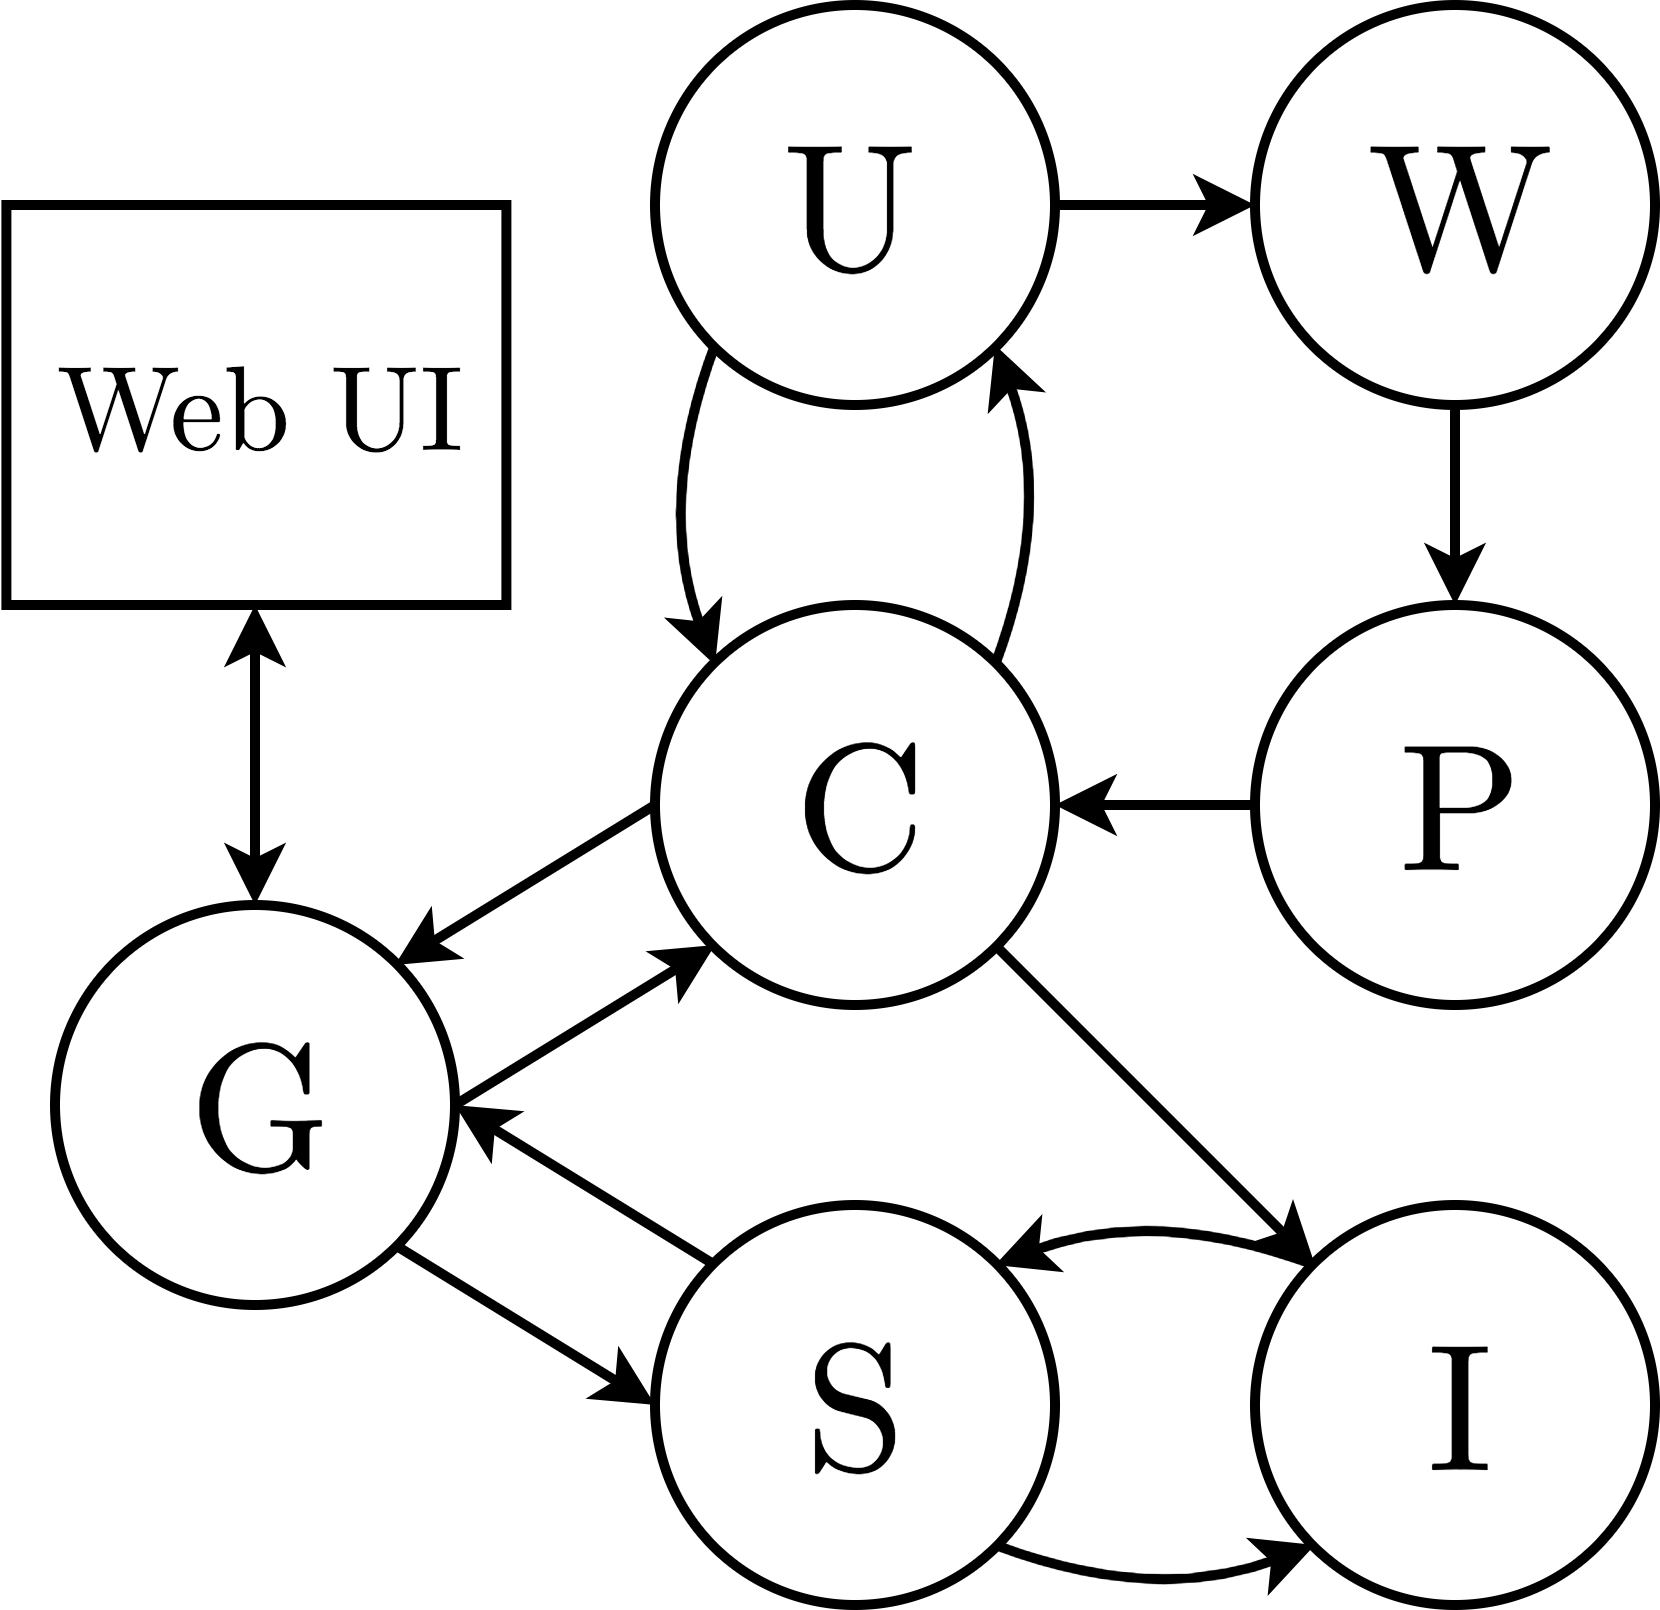
\includegraphics[width=0.7\textwidth]{graphics/interaction-model.png} 
      \caption{Interaction Model}
    \end{figure}
  \end{column}
\end{columns}

\end{frame}

% ###################################################################

\begin{frame}{Software Artifact Analysis}

\begin{table}
  \begin{tabular}{l|r|r|r|r}
    \textbf{Artifact} & \textbf{LoC} & \textbf{sJAR (KB)} & \textbf{fJAR (KB)} & \textbf{Up (s)}  \\ \hline
    Akka monolith     & 4487         & 1004.3             & 76 775.1           & 5.5                     \\ \hline
    CatalogStore (MS) & 1838         & 56.1               & 89 225.8           & 14.6                    \\ \hline
    IndexStore (MS)   & 724          & 23.8               & 83 518.2           & 8.8                     \\ \hline
    Searcher (MS)     & 656          & 22.2               & 81 754.4           & 8.1                     \\ \hline
    Web Crawler (MS)  & 716          & 23.5               & 83 517.9           & 9.2                     \\ \hline
    Parser (MS)       & 703          & 24.2               & 83 519.1           & 8.6                     \\ \hline
    Registry (MS)     & 334          & 9.9                & 90 699.7           & 9.4                     \\ \hline
    Gateway (MS)      & 889          & 30.5               & 83 655.1           & 9.7                     \\ \hline
    Updater (MS)      & 693          & 23.9               & 83 518.3           & 8.7                     \\ \hline
  \end{tabular}
\end{table}

\begin{itemize}
  \item $\sum\mbox{LoC}(\mbox{MS}) = 6553$, about 46 \% larger
\end{itemize}

\end{frame}

% ###################################################################

\begin{frame}{Artifact Memory Consumption}

Memory consumption of the executable artifact VMs in the indexing phase:

\begin{center}
  \begin{figure} 
    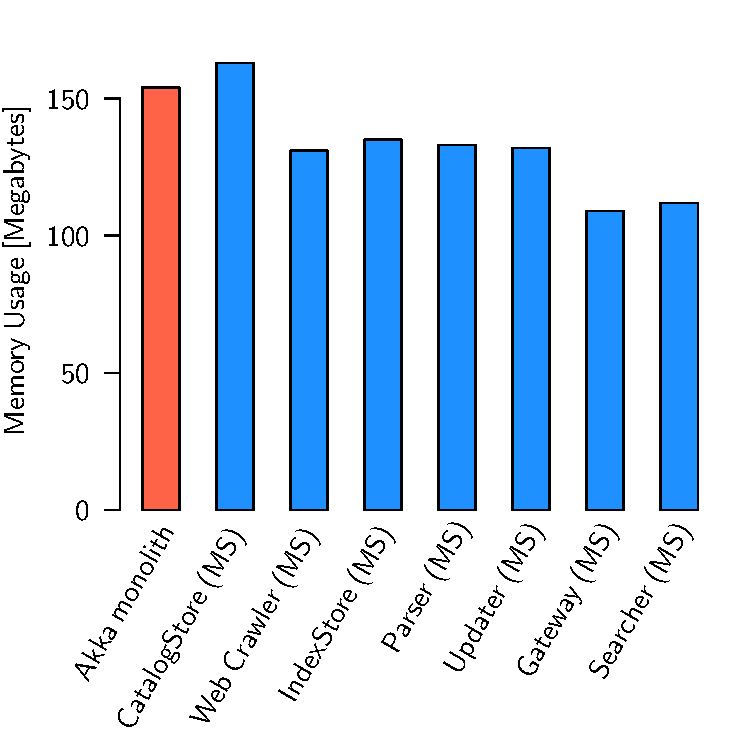
\includegraphics[width=0.5\textwidth]{graphics/eval-index-mem.pdf} 
  \end{figure}
\end{center}

\end{frame}

% ###################################################################

\begin{frame}{Overall Processing Time: Indexing Subsystem}

Benchmark results for the overall processing time of the indexing subsystem:

\begin{center}
  \begin{figure} 
    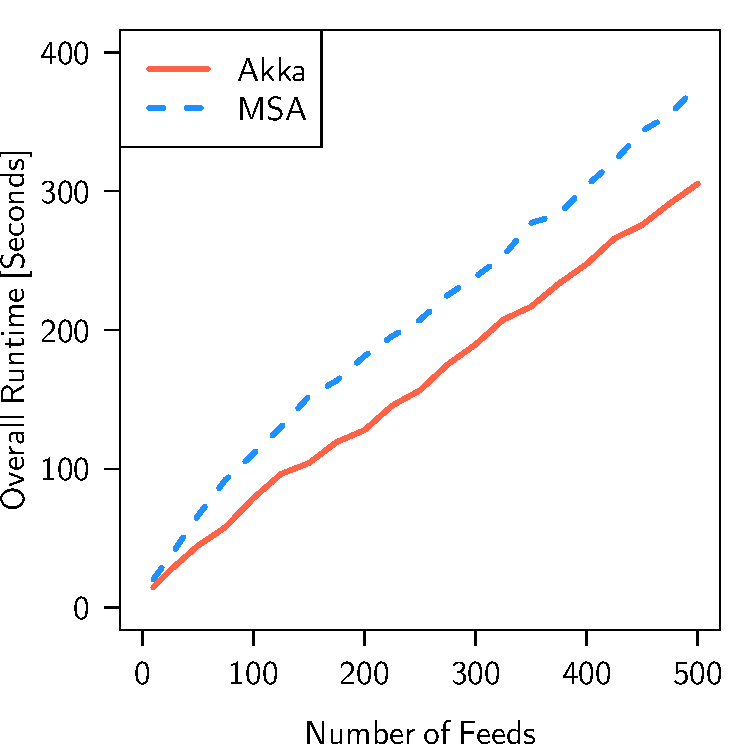
\includegraphics[width=0.5\textwidth]{graphics/eval-index-overall.pdf} 
  \end{figure}
\end{center}

\end{frame}

% ###################################################################

\begin{frame}{Overall Processing Time: Retrieval Subsystem}

Benchmark results of the overall processing time for the retrieval subsystem:

\begin{center}
  \begin{figure} 
    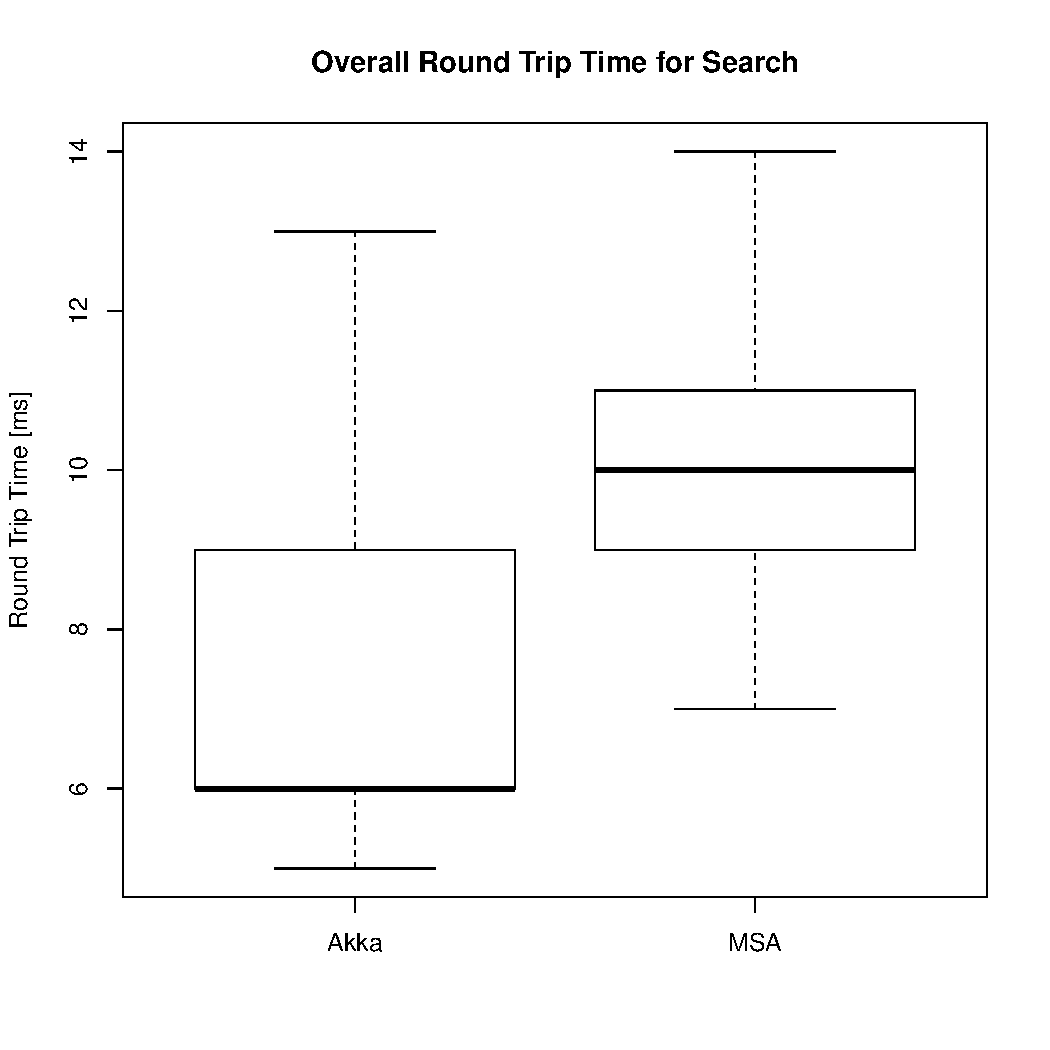
\includegraphics[width=0.5\textwidth]{graphics/eval-search-rtt-overall.pdf} 
  \end{figure}
\end{center}

\end{frame}

% ###################################################################

\begin{frame}{Contributions}

\begin{itemize}
  \item Compared the programming of concurrent computation with the actors and microservices
  \item Explored the interrelations of the two models and filled a gap in the literature
  \item Designed a non-trivial scenario for a concurrent domain-specific search engine
  \item Actor and microservice implementation
  \item Capability evaluation and efficiency benchmark
\end{itemize}

\end{frame}

% ###################################################################


\begin{frame}{}

\begin{center}
  \texttt{</end>}
\end{center}

\end{frame}

% ###################################################################

\begin{frame}{Supplemental: State Encapsulation vs. Isolation}

\begin{itemize}
  \item Microservice: process memory boundaries
  \item Actors (on the JVM):
  \begin{itemize}
    \item Visibility $+$ Accessibility $\rightarrow$ information hiding
    \item Reference types $+$ pass-by-value $\rightarrow$ immutability
    \item Coding conventions required
  \end{itemize}
\end{itemize}

\end{frame}

% ###################################################################

\begin{frame}[fragile]{Supplemental: Actor state isolation in Java}

\begin{verbatim}
public class Foo extends UntypedActor {
    public String bar;
    public static Props props() {
        return Props.create(Foo.class, () -> new Foo());
    }
    @Override
    public void onReceive(Object msg) { 
      /* handle msg */ 
    }
}

final ActorRef foo = system.actorOf(Foo.props());
\end{verbatim}

\end{frame}

% ###################################################################

\begin{frame}{Supplemental: Semi-Synchronous Communication in Akka}

Comparison of the benchmark results for the retrieval subsystem using either delegation or futures for request/response communication in the Akka:

\begin{center}
  \begin{figure} 
    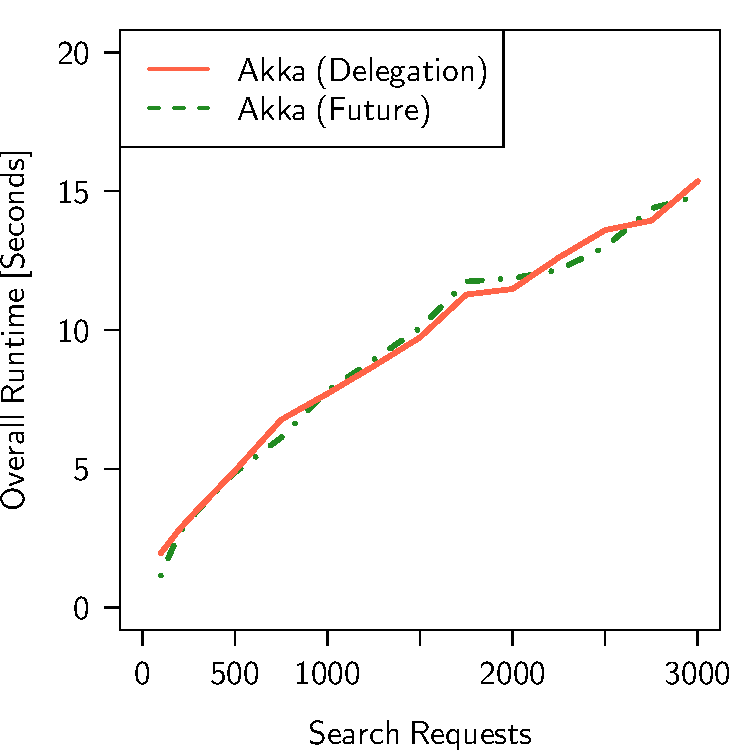
\includegraphics[width=0.5\textwidth]{graphics/eval-search-comparison-akka-delegation-future.pdf} 
  \end{figure}
\end{center}

\end{frame}

% ###################################################################

\begin{frame}{Supplemental: Relevance of the Benchmark}

\begin{itemize}
  \item First benchmark comparing Akka actors and Spring- based microservices (full application context)
  \item Lack of different interaction modes in microservice architecture benchmarks according to literature $\rightarrow$ comparison to asynchronous actor system
\end{itemize}

\end{frame}

% ###################################################################


\end{document}

